\section{Formalization}


\subsection{Formalization CPS ontology}
\label{for:CPS_ontology}
The formalization of a CPS is organized along multiple levels: (L1) aspects and concerns; (L2) properties; (L3) CPS configuration; (L4) actions; (L5) constraints, dependencies and trade-offs; and (L6) satisfaction axioms. Level L1 and L6 form the \emph{CPS-independent specification}, since aspects and concerns are independent of the specific CPS being modeled. Levels L2-L5 comprise the \emph{CPS-dependent specification}, as the information included in them depends on the CPS being modeled. Furthermore, levels L1 and L2 formalize the concepts from the definition of the CPS Framework. Levels L3-L5 extend the CPS Framework in order to provide details needed for reasoning about the behavior of a CPS of interest. Level L6 provides the semantics of the formalization. The ASP representation for 6 levels of CPS ontology is described in section ~\ref{sub-section:asp_representation}

\subsection{A Physical CPS System}
\label{for:physical_CPS_system}
\begin{definition}
\label{def:physical_CPS_system} 
A physical CPS system $S$ is a tuple ($C, A, F, R$) where:
%
\begin{list}{$\bullet$}{\itemsep=0pt \parsep=1pt \topsep=1pt \leftmargin=12pt} 
\item $C$ is a set of physical components.
\item $A$ is a finite set of actions that can be execute over CPS system.
\item $F$ is a finite set of fluent literals.
\item $R$ is a set of relations that map each physical component $c \in C$ with a set of physical component properties that are defined in CPS Ontology.  \\
For any $r \in R$, $r : C \longrightarrow 2^{P_{C}}$. In which, we have $2^{P_{C}}$ is power set of $P_{C}$, $P_{C}$ is set of properties which related to physical components, $P$ is set of all properties that are defined in CPS ontology ~\ref{sub-section:CPS_ontology} and $P_{C} \subset P$. 
\end{list}
%
\end{definition}
%
Intuitively, the CPS problem related the example in use case ~\ref{sub-section:use_case} can be specified by $S_{auto} = $ ($C_{auto}, A_{auto}, F_{auto}, R_{auto}$) where:
\begin{list}{$\bullet$}{\itemsep=0pt \parsep=1pt \topsep=1pt \leftmargin=12pt} 
\item $C_{auto} = \{{\tt SAM}, {\tt CAM}\}$ .
\item $A_{auto}$ is set of finite actions which consists of:
\begin{list}{$\bullet$}{\itemsep=0pt \parsep=1pt \topsep=1pt \leftmargin=12pt} 
\item {\tt \small switMem(X,encrypted),switMem(X,unencrypted)}: denote actions to switch component $X$ using encrypted or unencrypted memory respectively. 
\item {\tt \small switReMod(X,50fps),switReMod(X,25fps)}: denote actions to switch component $X$ using 50 fps and 25 fps recording modes respectively. 
\item {\tt \small switModel(X,basic),switReMod(X,advanced)}: denote actions to switch component $X$ using basic and advanced models respectively. 
\item etc. (should be more)
\end{list}
\item $F_{auto}$ is a finite set of fluent literals which consists of:
\begin{list}{$\bullet$}{\itemsep=0pt \parsep=1pt \topsep=1pt \leftmargin=12pt} 
\item {\tt \small useMem(X,encrypted),useMem(X,unencrypted)}: denote that component $X$ is using encrypted or unencrypted memory respectively. 
\item {\tt \small recordMode(X,50fps),recordMode(X,25fps)}: denote that component $X$ is recording video with 50 fps and 25 fps modes respectively. 
\item {\tt \small useModel(X,basic),useModel(X,advanced)}: denote that component $X$ is working on basic and advanced models respectively. 
\item etc. (should be more)
\end{list}
\item $R_{auto} =\{${\tt CAM} $\mapsto \{{\tt reMode\_50fps, model\_basic,...}\}$, {\tt SAM} $\mapsto \{{\tt mem\_encrypted, boot\_sec,...}\}$  $\}$ \\
In which, {\tt \small reMode\_50fps, reMode\_25fps, model\_basic, mem\_encrypted, boot\_sec, etc.}  are defined in CPS Ontology properties ~\ref{sub-section:CPS_ontology}. 
\end{list}
\subsection{Truthworthiness Problem Definition}
\emph{Truthworthiness} is one of nine highest level concerns (\emph{aspects}) and a critical concern stakeholders have about CPS and the Internet of Things (IoT) and their development.There, \emph{trustworthiness} is captured as a high-level concern encompassing safety, security, privacy, resilience, and reliability. While there are many efforts, in multiple sectors, to study these characteristics of systems they are typically considered separately and in isolation. This can result in work, intended to address one of these concerns, adversely impacting work to address one or more of the others. Thus CPS/IoT trustworthiness relies on an integrated, concern-driven approach that takes into account the interactions between the cyber and physical elements of systems. There are some important \emph{Truthworthiness} queries which should be answered in CPS system: 
\begin{itemize}
	\item Is the Truthworthiness aspect satisfied? 
	\item What is the most vulnerability in CPS system?
	\item If there exists the vulnerability in CPS system, how to fix it?
\end{itemize}
\begin{figure}
	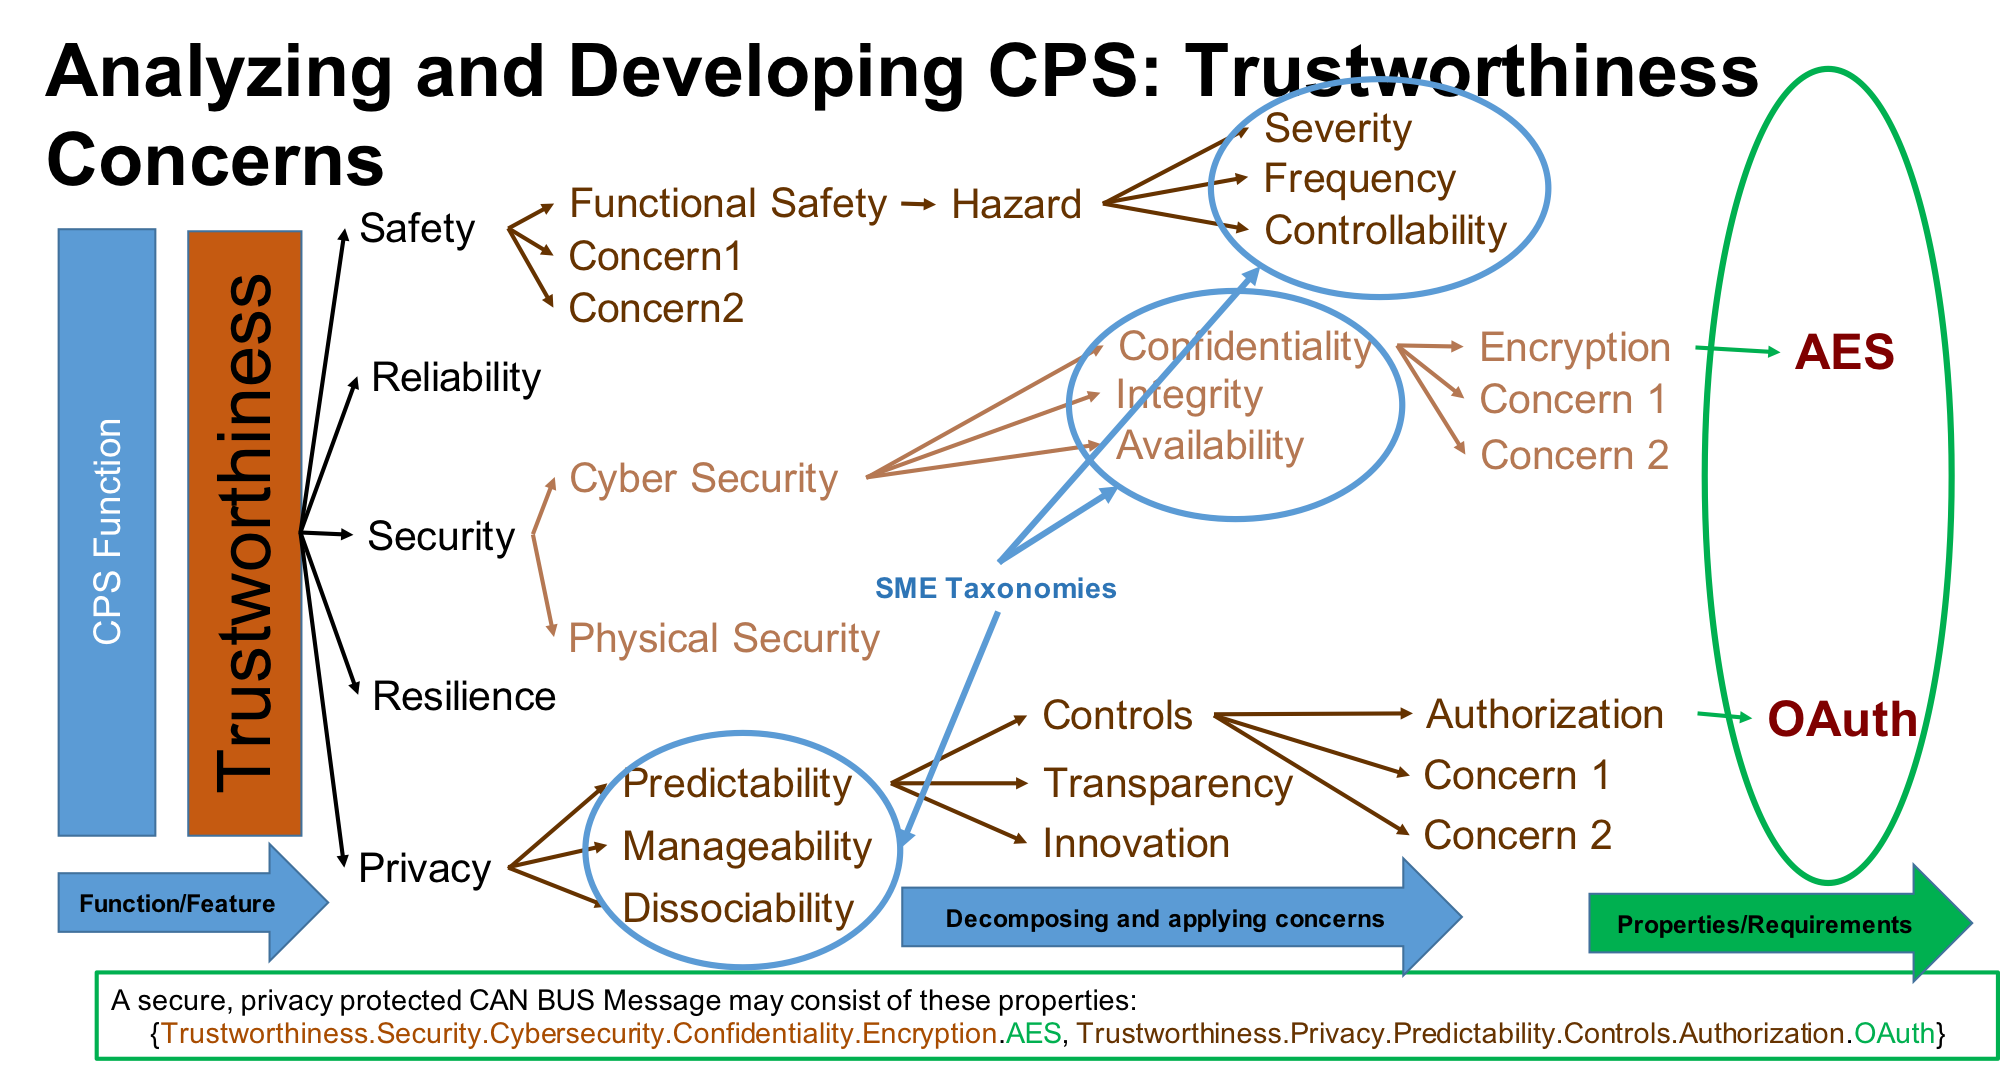
\includegraphics[width=250pt]{trustconcerntree.png}
	\caption{Decomposition tree for Trustworthiness Concerns\label{fig:trustworthiness}}
\end{figure}

\subsection{Probability of success of mitigation strategies}
\begin{definition}
	\label{def:probability_of_success} 
	
\end{definition}

\subsection{Likelihood of Concerns Satisfaction}
\begin{definition}
	\label{def:likelihood_concern_sat} 
	
\end{definition}

\subsection{Vulnerability in CPS System}
\begin{definition}
	\label{def:vulnerability} 
	
\end{definition}

\begin{proposition}
	\label{pro:most_vulnerability} 
	
\end{proposition}